\documentclass[a4paper, 12pt]{article}%тип документа

%отступы
\usepackage[left=2cm,right=2cm,top=2cm,bottom=3cm,bindingoffset=0cm]{geometry}

%Русский язык
\usepackage[T2A]{fontenc} %кодировка
\usepackage[utf8]{inputenc} %кодировка исходного кода
\usepackage[english,russian]{babel} %локализация и переносы

%Вставка картинок
\usepackage{wrapfig}
\usepackage{graphicx}
\graphicspath{{pictures/}}
\DeclareGraphicsExtensions{.pdf,.png,.jpg}

%оглавление
\usepackage{titlesec}
\titlespacing{\chapter}{0pt}{-30pt}{12pt}
\titlespacing{\section}{\parindent}{5mm}{5mm}
\titlespacing{\subsection}{\parindent}{5mm}{5mm}
\usepackage{setspace}

%Графики
\usepackage{multirow}
\usepackage{pgfplots}
\pgfplotsset{compat=1.9}

%Математика
\usepackage{amsmath, amsfonts, amssymb, amsthm, mathtools}

%Стиль страницы
\usepackage{fancyhdr}
\pagestyle{fancy}

\begin{document}

\begin{titlepage}

\begin{center}
%\vspace*{1cm}
\large\textbf{Московский Физико-Технический Институт}\\
\large\textbf{(государственный университет)}
\vfill
\line(1,0){430}\\[1mm]
\huge\textbf{Работа 4.1.2.}\\
\line(1,0){430}\\[1mm]
\vfill
\large Сибгатуллин Булат, ФРКТ\\
\end{center}

\end{titlepage}
\fancyhead[L] {Работа 4.1.2.}
\noindent \textbf{Цель работы:} \\
\indent Определить фокусные расстояния собирающих и рассеивающих линз, смоделировать ход лучей в трубе Галилея, трубе Кеплера и микроскопе, определить их увеличение.\\
\noindent \textbf{В работе используются:} \\
\indent оптическая скамья, набор линз, экран, осветитель со шкалой, зрительная труба, диафрагма, линейка.

\section*{Экспериментальная установка}

Набор линз, осветитель, экран, зрительная труба, необходимые для моделирования оптических приборов, устанавливаются при помощи рейтеров на оптической скамье. Предметом служит
	миллиметровая шкала или сетка, нанесённая на матовое стекло осветителя.
	
	\section*{Центрирование линз.} При юстировке любых оптических приборов важно правильно центрировать входящие в систему линзы. Проходя через плохо
	отцентрированную систему линз, лучи света отклоняются в сторону и могут
	вообще не доходить до глаза наблюдателя. Центрировать линзы следует как
	по высоте, так и в поперечном направлении (для чего линзы крепятся на, поперечных салазках). Подробно с правилами центрировки Вы познакомитесь
	при выполнении задания.
	
	\section*{Юстировка коллиматора.} При составлении моделей телескопических
	систем необходимо иметь удалённый объект. В качестве такого объекта обычно используется бесконечно удалённое изображение предмета (шкалы осветителя), установленного в фокальной плоскости положительной линзы. Лучи,
	выходящие из одной точки предмета, пройдя через линзу, образуют параллельный пучок. Устройство такого рода называется \textit{коллиматором}.

	Для юстировки коллиматора удобно использовать вспомогательную зрительную трубу, предварительно настроенную на бесконечность. Передвигая
	линзу коллиматора вдоль скамьи, добиваются появления резкого изображения предмета в окуляре зрительной трубы.
	
	\section*{Измерение фокусных расстояний линз.} Для того, чтобы сознательно
	моделировать оптические инструменты, нужно знать фокусные расстояния
	линз, которые могут быть использованы в качестве объектива или окуляра модели. Фокусные расстояния тонких положительных линз проще всего
	найти с помощью вспомогательной зрительной трубы, установленной на, бесконечность. Работа выполняется так же, как при юстировке коллиматора.
	
	При определении фокусного расстояния отрицательной линзы предметом
	служит изображение шкалы, которое даёт вспомогательная положительная
	линза.
	
	\begin{figure}
			\begin{center}
				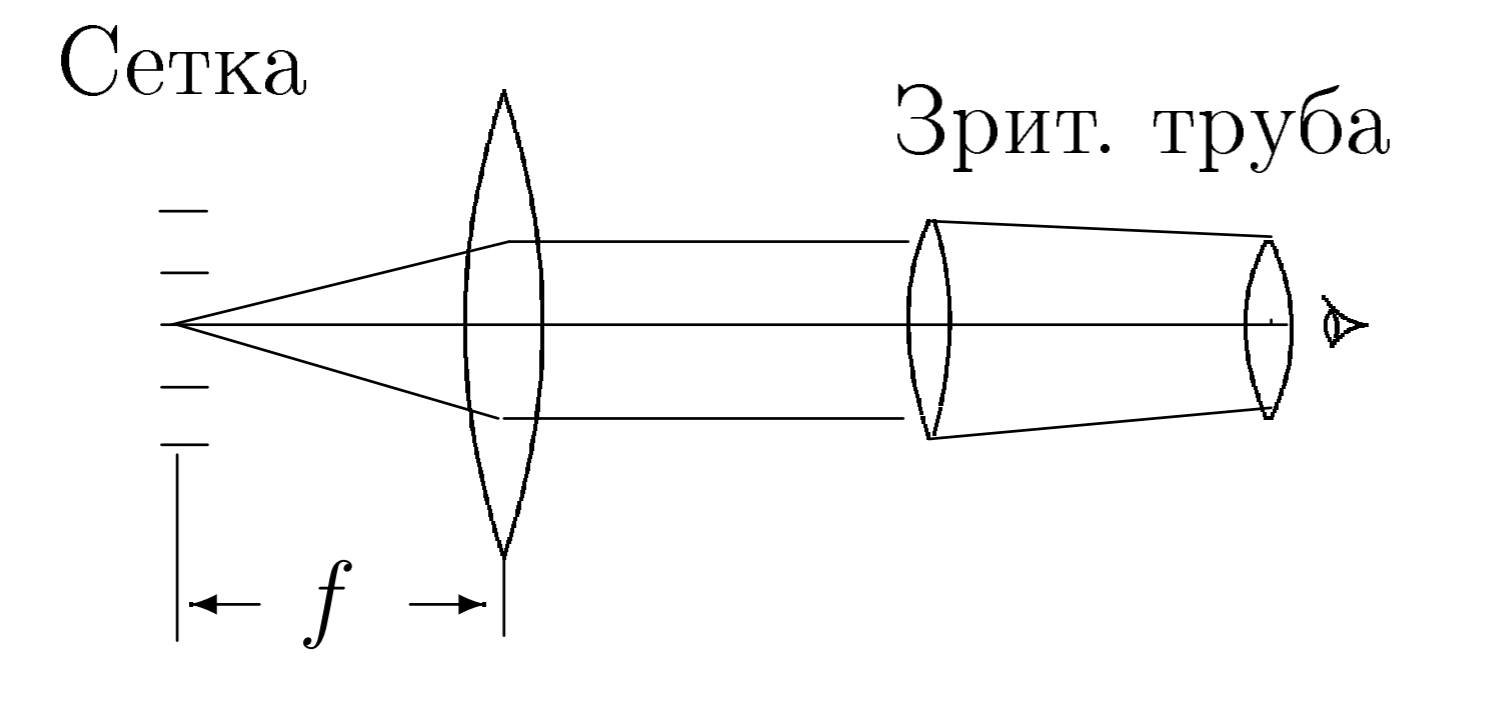
\includegraphics[width = 0.5\textwidth]{images/412-1.png}
				\caption{Определение фокусного расстояния собирающей линзы}
			\end{center}
		\end{figure}
		
	\begin{figure}
			\begin{center}
				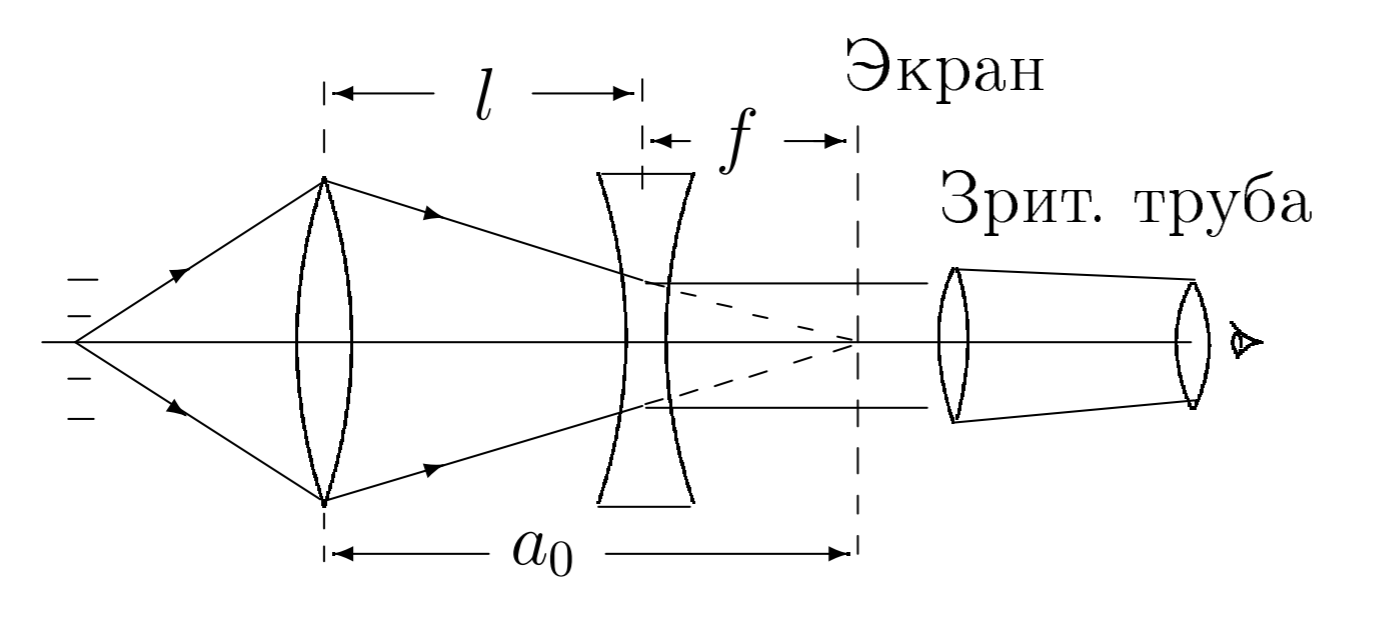
\includegraphics[width = 0.5\textwidth]{images/412-2.png}
				\caption{Определение фокусного расстояния рассеивающей линзы}
			\end{center}
		\end{figure}
		
	\begin{figure}
			\begin{center}
				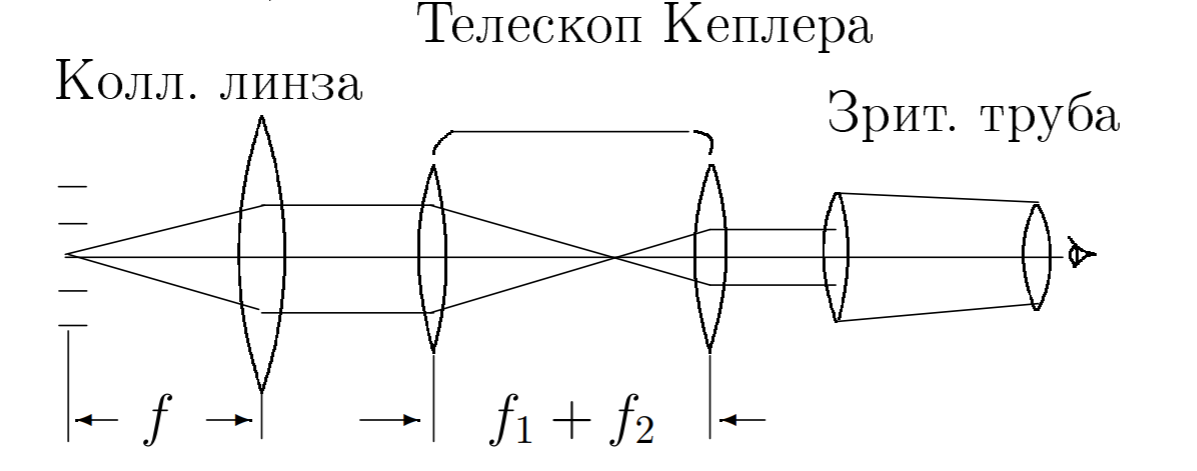
\includegraphics[width = 0.5\textwidth]{images/412-3.png}
				\caption{Модель телескопа}
			\end{center}
		\end{figure}
		
	\begin{figure}
			\begin{center}
				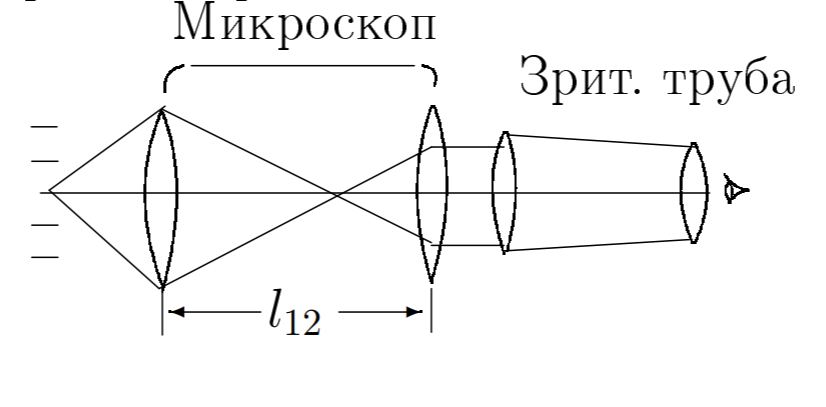
\includegraphics[width = 0.5\textwidth]{images/412-4.png}
				\caption{Модель микроскопа}
			\end{center}
		\end{figure}

\end{document}